\chapter{Prostate Cancer Detection Setting}

According to the Masaryk Memorial Cancer Institute in \cite{mmci-prostate-cancer}, prostate cancer is the most common oncological disease among men in the Czech Republic, with approximately $8$ thousand new cases reported each year.
In the global context, experts estimate $1,276,106$ of new cases appeared in $2018$ alone, per \cite{world-prostate-cancer}.
To aid pathologists in tackling the ever-growing number of new cases, the RationAI team trained and tested a CNN on a dataset provided by Masaryk Memorial Cancer Institute.

This chapter briefly introduces prostate cancer, a contemporary approach to detecting malignant tissue, and finally presents a dataset and RationAI's model for prostate cancer detection.

\section{Prostate Cancer}

Prostate cancer is a disease that causes rapid growth of cells in the prostate -- a male gland located under the bladder.
This gland produces seminal fluid, which helps transport and nourish sperm.
The type of cancer that attacks the glandular tissue is called adenocarcinoma.

Doctors commonly diagnose prostate cancer in men after the age of $50$, and the incidence rate keeps increasing with age --- we detect nearly $60$\% presence in men over $65$.
The mortality rate per $100,000$ people varies worldwide, ranging from $3.3$ in East Asia to $10.7$ in Central America. Diet, physical activity, ethnicity, and family history are all likely to influence the development and progression of cancer.
Implications of prostate cancer are significant even if it does not result in death, as it affects one's quality of life due to potential urinary, bowel, and sexual dysfunctions.
In advanced stages, prostate cancer can spread beyond the prostate gland and affect the bladder, rectum, or bones \cite{world-prostate-cancer}.
Given its high prevalence and potential for aggressiveness, early detection and effective treatment of prostate cancer are vital to improve outcomes and survival rates.

\subsection*{Gleason Patterns and Score}

In 1996, Donald Gleason introduced a unified grading and scoring system to effectively detect and assess the impact of adenocarcinoma spread in the prostate.
Gleason's system gained acceptance in 1974 and is the most prevalent system doctors use today.
It categorizes the growth of cancer cells into distinct patterns based on how much the cancerous tissue differs from healthy prostate gland cells, as shown in \myref{Figure}{fig:gp}.
Several patterns and their descriptions have since been refined, and we now distinguish between 9 patterns.
A full list and description of the patterns can be found in \cite{gleason-patterns}.

To calculate a Gleason score, the histopathologist determines the predominant and second most common Gleason pattern -- the final score is simply a sum of the pattern category numbers.
The International Society of Urological Pathology distinguishes between $5$ grades of prostate cancer.
For more on scoring and grading innuendos, see \cite{gleason-pattern-grading}.
In 2016, the World Health Organization refined the grading into so-called \emph{grade groups}, summarized in \cite{who-grade-groups}.

\begin{figure}
    \begin{center}
    \begin{minipage}{1\textwidth}
    \fcolorbox{RoyalBlue}{white}
      {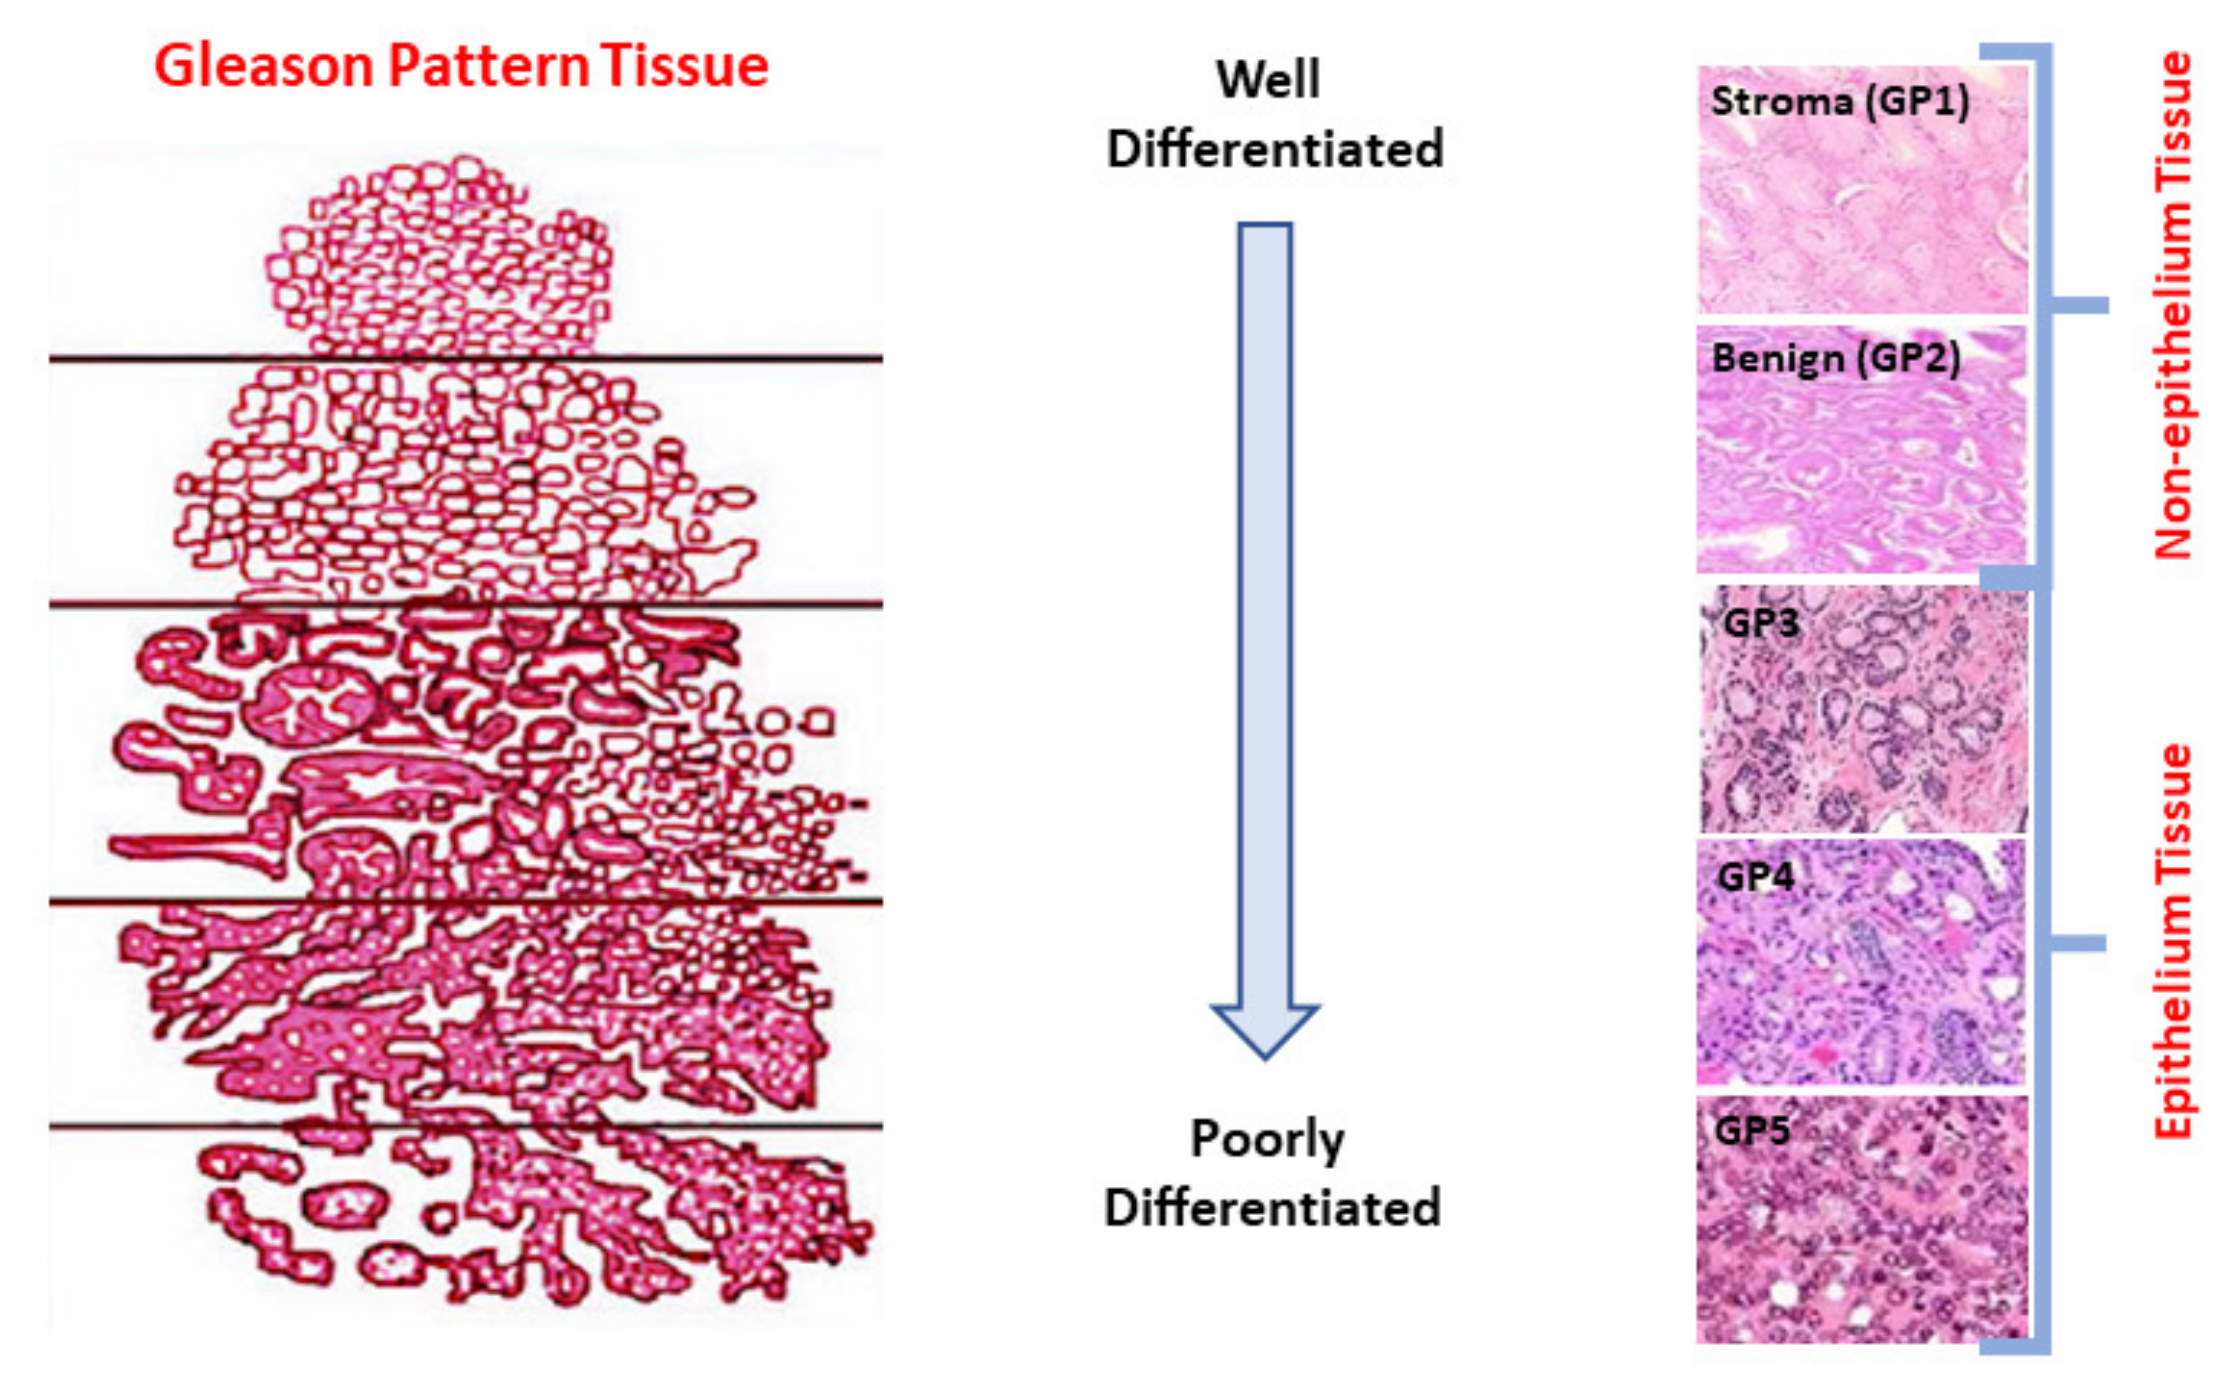
\includegraphics[width=\textwidth]{img/gp-classification.png}}
    \end{minipage}
    \caption{Example of Gleason Patterns ranked from $1$ to $5$. Pattern $1$ represents a healthy stroma --- ``cells and tissues that support and give structure to organs, glands, or other tissues in the body'', per definition from \cite{nci-stroma}. Pattern $5$ represents tissue with the highest risk of cancer. Sourced from \cite{gleason-pattern-description}.}
    \label{fig:gp}
    \end{center}
\end{figure}

\section{Dataset}\label{sec:dataset}

The Masaryk Memorial Cancer Institute provided the RationAI group with a pseudonymized dataset of hematoxylin/eosin-stained WSIs.
Each WSI contains $3$ to $5$ biopsies and is stored as an uncompressed PNG of size $105,185 \times 221,772$ pixels.
The dataset is stratified into training and test splits, containing $264$ WSIs with cancer, $436$ without, $37$ WSIs with cancer, and $50$ without, respectively \cite{gallo}.
To mark cancerous areas, domain experts manually annotated areas of WSIs containing adenocarcinomas -- annotations are polygons encapsulating cancerous regions.
\myref{Table}{tab:who_grade_distribution} shows the WHO grade group distribution.

\begin{table}
\centering
\ra{1.2}
\begin{tabular}{@{} l r r @{}}\toprule
WHO Grade Distribution & Training split & Test split \\ 
\midrule
Grade 1         & 38 cases            & 5 cases      \\
Grade 2         & 31 cases            & 1 case       \\
Grade 3         & 16 cases            & 1 case       \\
Grade 4         & 9 cases             & 1 case       \\
Grade 5         & 10 cases            & 2 case       \\
\bottomrule
\end{tabular}
\caption{WHO grade distributions for the training and test splits of the prostate WSI dataset. The test split consists of $87$ biopsies from 10 patients and is intended to ``represent different Gleason patterns
and types of infiltration'' \cite{gallo}, loosely copying the distribution of the training split. While each case is from a patient with a positive diagnosis, some of the biopsies do not contain cancer, so the positive/negative ratio is $37/50$.}
\label{tab:who_grade_distribution}
\end{table}

WSIs come with a so-called pyramid structure, which consists of multiple layers of the same image at different resolutions, each representing a deeper level of magnification.
As the user zooms in on a particular area of the slide, higher resolution layers of the pyramid are rendered, providing more detail without compromising loading times.
Because processing the entire WSI at once is computationally expensive, we tile the WSIs to reduce memory requirements.
Each WSI is divided into overlapping tiles of size $512 \times 512$ pixels.
An overlap of $256$ pixels is used between two consecutive tiles to counteract the possibility of severing critical patterns.
We cut out tiles at a resolution of $0.344$ \si{\micro\meter} per pixel, which corresponds to a $10$ times magnification.

Since WSIs contain multiple biopsies with gaps in between them, we chisel out only relevant parts.
Any tile with less than $50$\% of its area covered by tissue is discarded from the training and test dataset splits.
Consequently, although all WSIs are the same size, the number of usable tiles per slide is different.

\section{Model}\label{model}

A model trained by the RationAI group to perform cancer detection in tiled WSIs is a modified version of the well-known CNN architecture VGG16, introduced in \cite{vgg16}.
\myref{Figure}{fig:rationai-vgg16} shows the full model decomposition.

Loosely paraphrasing \cite{gallo}, the model aims to solve the following problem: \emph{Classify tiles according to the presence/absence of cancer in their central square area of $256 \times 256 $ pixels. Presence is determined by whether the central square overlaps with the domain expert's annotation}. The model performs remarkably well on the test split, reaching $100$\% slide-level prediction accuracy --- that is, the model correctly determines whether a WSI contains cancer for each test WSI.

However, in a high-stakes environment such as cancer detection, it is not enough to blindly trust the model based on accuracy.
To verify that the model bases its decisions on relevant features, Gallo et at. performed an additional experiment in \cite{gallo}, presenting a subset of the dataset from \myref{Section}{sec:dataset} including regions of models' interest annotated by the technique described in \myref{Section}{occlusion} to a domain expert.
The domain expert concluded that the model focuses on critical morphological features \cite{gallo} on which human pathologists would base their decisions.

\begin{figure}
    \begin{center}
    \begin{minipage}{0.75\textwidth}
      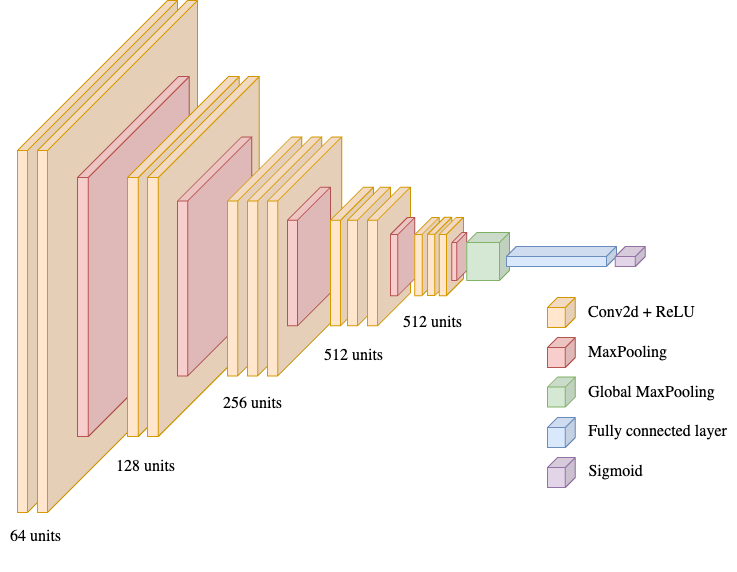
\includegraphics[width=\textwidth]{img/nn-arch.png}
    \end{minipage}
    \caption{Architecture of Prostate Cancer Binary Classifier model utilized by the RationAI group. The model is based on VGG16, introduced by Simonyan and Zisserman in \cite{vgg16}. They originally trained their VGG16 model to classify $1000$ classes from the ILSVRC dataset \cite{ilsvrc} and utilized three FC layers before applying softmax on the last one. RationAIs' solution places global max pooling before a single FC layer, reducing each of the $512$ pooled activation maps to a single value. Sigmoid is applied to the output of the FC layer to squish the raw value in the range $(0, 1)$. Therefore, we can interpret the final output as a probability of pro-cancer markers in a given tile's central $256 \times 256$ pixel square.}
    \label{fig:rationai-vgg16}
    \end{center}
\end{figure}

